\themaM
\graphicspath{{../Ch14_Durees_et_masses/Images/}}

\chapter{Durées}
\label{C22}


%%%%%%%%%%%%%%%%%%%%%%%%%%%%%%%%%%%%%%%%%%
\begin{prerequis}[Connaissances et compétences abordées]
   \begin{itemize}
      \item Calculer la durée écoulée entre deux instants donnés.
      \item Déterminer un instant à partir de la connaissance d’un instant et d’une durée.
      \item Connaître et utiliser les unités de mesure des durées et leurs relations : unités de mesures usuelles (jour, semaine, heure, minute, seconde, dixième de seconde, mois, année, siècle, millénaire).
      \item Résoudre des problèmes en exploitant des ressources variées (horaires de transport, horaires de marées, programmes de cinéma ou de télévision, etc.).
   \end{itemize}
\end{prerequis}

\vfill

\begin{debat}[Débat : instruments anciens de mesure de temps et de durée]
   De tous temps on a voulu mesurer le {\bf temps} et la {\bf durée}, ci-dessous figurent quelques instruments utilisés dans des époques plus ou moins lointaines : \\
   \textcolor{B1}{\small
   \begin{tabular}{*{4}{C{3.5}}}
      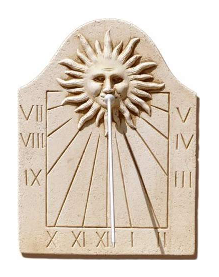
\includegraphics[width=2.8cm]{cadran}
      &
      \includegraphics[width=2.8cm]{nocturlabe}
      &
      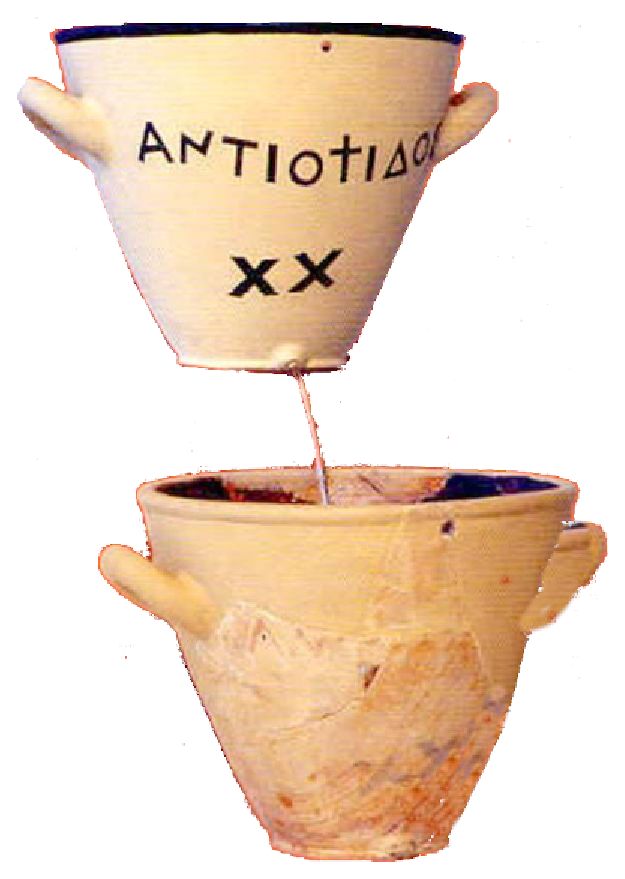
\includegraphics[width=2.8cm]{clepshydre}
      &
      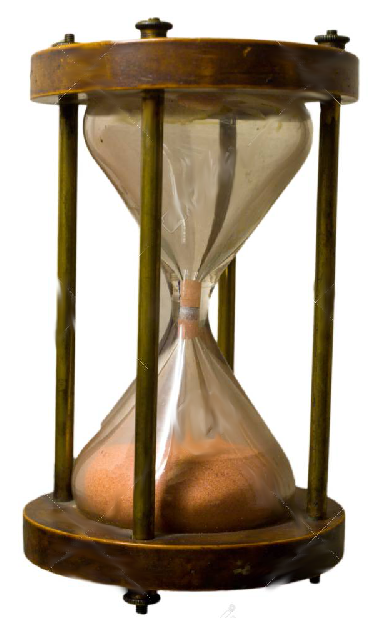
\includegraphics[width=2.8cm]{sablier} \\
      Cadran solaire & Nocturlabe & Clepsydre & Sablier \\
      1\,500 av. J.-C. & X\up{e} siècle & 1\,600 av. J.-C. & IX\up{e} siècle \\
      Heures du jour & Heures de la nuit & Durées longues (heures) & Durées courtes (minutes) \\
   \end{tabular}}
   \bigskip
   \begin{cadre}[B2][F4]
      \begin{center}
         Vidéo : \href{https://www.youtube.com/watch?v=8vMTE9U9z0U}{\bf Remettons les pendules à l'heure}, chaîne YouTube {\it C'est pas sorcier}.
      \end{center}
   \end{cadre}
\end{debat}

\vfill

\textcolor{PartieGeometrie}{\sffamily\bfseries Cahier de compétences} : chapitre 2, exercices 45 à 57 ; 62 à 64.


%%%%%%%%%%%%%%%%%%%%%%%%%%%%%%%%%%%%
%%%%%%%%%%%%%%%%%%%%%%%%%%%%%%%%%%%%
\activites

\begin{activite}[De la seconde au siècle]
   {\bf Objectif :} ordre de grandeur dans le domaine des durées. 
   \begin{QCM}
      Relier les durées suivantes à son ordre de grandeur de durée.
      \begin{center}
         {\psset{yunit=0.9}
         \small
         \begin{pspicture}(-8,-11)(8,11)
            {\normalsize
            \rput(0,9){Siècle}
            \rput(0,6){Année}
            \rput(0,3){Mois}
            \rput(0,0){Jour}
            \rput(0,-3){Heure}
            \rput(0,-6){Minute}
            \rput(0,-9){Seconde}}
            \psdots(-1.5,-9)(-1.5,-6)(-1.5,-3)(-1.5,0)(-1.5,3)(-1.5,6)(-1.5,9)(1.5,-9)(1.5,-6)(1.5,-3)(1.5,0)(1.5,3)(1.5,6)(1.5,9)(-4,-10)(-4,-6)(-4,-2)(4,2)(4,6)(4,10)(4,-10)(4,-6)(4,-2)(-4,2)(-4,6)(-4,10)
            \rput(-6.25,-6){\parbox{3.5cm}{Temps mis par la lumière pour parcourir une distance équivalente à celle séparant la Terre et la Lune.}}
            \rput(6.25,2){\parbox{3.5cm}{Durée d'une saison.}}
            \rput(-6.25,2){\parbox{3.5cm}{Record du monde du \um{100}.}}
            \rput(-6.25,-2){\parbox{3.5cm}{Temps de cuisson d'un \oe uf à la coque.}}
            \rput(6.25,6){\parbox{3.5cm}{Intervalle entre deux battements de c\oe ur consécutifs.}}
            \rput(-6.25,10){\parbox{3.5cm}{Durée d'un cycle complet de lune.}}
            \rput(6.25,-6){\parbox{3.5cm}{Durée d'un film.}}
            \rput(6.25,-10){\parbox{3.5cm}{Temps mis par la Terre pour faire le tour de son étoile le Soleil.}}
            \rput(6.25,10){\parbox{3.5cm}{Age maximum atteint par un humain.}}
            \rput(-6.25,6){\parbox{3.5cm}{Durée d'une grossesse.}}
            \rput(6.25,-2){\parbox{3.5cm}{Durée d'un entraînement de sport.}}
            \rput(-6.25,-10){\parbox{3.5cm}{Durée d'un weekend.}}
            \multido{\n=-9+3}{7}{\rput(0,\n){\psframe(-1,-0.5)(1,0.5)}}
         \end{pspicture}}
      \end{center}
   \end{QCM}
\end{activite}


%%%%%%%%%%%%%%%%%%%%%%%%%%%%%%%%%%%%%%%%%%
\cours 

%%%%%%%%%%%%%%%%%%%%%%%%%%%%%%%%%%%%%%
\section{Unités de temps}

   Selon les situations, on utilise des unités de durées différentes selon les correspondances suivantes :
   
   \begin{multicols}{2}
      $\textcolor{A1}{\bullet}$ 1 millénaire = 10 siècles = 10$\times$100 ans = 1\,000 ans ; \\ 
      $\textcolor{A1}{\bullet}$ 1 an = 12 mois = 365 jours ou 366 jours ; \\
      $\textcolor{A1}{\bullet}$ 1 mois =  28 jours, 29 jours, 30 jours ou 31 jours ; \\
      $\textcolor{A1}{\bullet}$ 1 jour = 24 heures ; \\
      $\textcolor{A1}{\bullet}$ 1 heure = 60 minutes = 3\,600 secondes ; \\
      $\textcolor{A1}{\bullet}$ 1 seconde = 10$\times$1 dixième de seconde. 
   \end{multicols}

\begin{remarque}
   de manière générale, le système d'unités de durées n'est pas décimal, sauf pour les durées inférieures à la seconde (dixièmes, centièmes de secondes). \\
   Par exemple, une heure et demi  peut s'écrire 1,5 h = 1 h 30 min $\neq$ 1,3 h.
\end{remarque}


%%%%%%%%%%%%%%%%%%%%%%%%%%%%%%%%%%%%
\section{Conversion de durées}

\begin{methode*2*2}
   Pour convertir des heures en minutes ou des minutes en secondes ou inversement, on peut utiliser le schéma suivant : \\
   {\psset{xunit=0.8,yunit=0.6}
   \footnotesize
   \begin{pspicture}(-2.7,-3.7)(5,3.7)
      \ovalnode{A}{durée en heures}
      \ovalnode{B}{durée en minutes}
      \ovalnode{C}{durée en secondes}
      \nccurve[angle=90,linecolor=B1]{->}{A}{B}
      \ncput*{\textcolor{B1}{$\times 60$}}
      \nccurve[angle=90,linecolor=B1]{->}{B}{C}
      \ncput*{\textcolor{B1}{$\times 60$}}
      \nccurve[angle=-90,linecolor=A1]{->}{B}{A}
      \ncput*{\textcolor{A1}{$\div 60$}}
      \nccurve[angle=-90,linecolor=A1]{->}{C}{B}
      \ncput*{\textcolor{A1}{$\div 60$}}
      \nccurve[angle=90,linecolor=B1]{->}{A}{C}
      \ncput*{\textcolor{B1}{$\times 3\,600$}}
      \nccurve[angle=-90,linecolor=A1]{->}{A}{C}
      \ncput*{\textcolor{A1}{$\div 3\,600$} }
   \end{pspicture}}
   \exercice
       Convertir 170 minutes en heures et minutes.     
   \correction
      $170=2\times60+50$, donc \\
      170 min = 2 h 50 min.
   \exercice
      Convertir 1 h 25 min 36 s en secondes.
   \correction
      1 h = 3\,600 s et 1 min = 60 s donc \\
      1 h 25 min 36 s = 3\,600\ s + $25\times60$ s + 36 s = 5\,136 s.
\end{methode*2*2}

\bigskip

Pour effectuer des additions ou soustractions, on peut effectuer une opération experte (un peu périlleuse) ou procéder de proche en proche.
 
\begin{exemple}
\ \\ [-10mm]
  \begin{itemize}
      \item Un train part de Montpellier à 8 h 48. La durée du trajet pour se rendre à Paris est de 3 h et 20 min. \\
      À quelle heure arrivera-t-il à Paris ?
      \item Un automobiliste part de Montpellier à 8 h 35 et arrive à Perpignan à 10 h 20. \\
   Quelle est la durée de son trajet ?
   \end{itemize}
\correction
\ \\ [-10mm]
   \begin{itemize}
      \item   
      \begin{tabular}{C{0.5}ccccc}
         & & 8 & h & 4 & 8 \\
         & $+$ & 3 & h & 2 & 0 \\
         \hline
         & 1 & $\cancel{1}$ & h & $\cancel{6}$ & 8 \\
         = & 1 & 2 & h & 0 & 8 \\
      \end{tabular}
      \item 8 h 35 \quad $\xrightarrow{+\text{25 minutes}}$ \quad 9 h 00 \\
      9 h 00 \quad $\xrightarrow{+\text{1 heure}}$ \quad 10 h 00 \\
      10 h 00\quad $\xrightarrow{+\text{20 minutes}}$ \quad 10 h 20. \\   
      La durée totale du trajet est de 1 h 45.
   \end{itemize}   
\end{exemple}


%%%%%%%%%%%%%%%%%%%%%%%%%%%%%%%%
%%%%%%%%%%%%%%%%%%%%%%%%%%%%%%%%
\exercicesbase

\begin{colonne*exercice}

\serie{Conversion et calcul de durées} %%%%%

\begin{exercice}
   Convertir les durées en heures et minutes.
   \begin{enumerate}
      \item 1,5 h.
      \item 2,25h.
      \item 0,3h.
   \end{enumerate}
\end{exercice}

\begin{exercice}
   Convertir les durées en heures décimales.
   \begin{enumerate}
      \item 1 h 30 min.
      \item 2 h 45 min
      \item 8 h 15 min.
   \end{enumerate}
\end{exercice}
 
\begin{exercice}
   Convertir les durées en minutes.
   \begin{enumerate}
      \item 1 h 56 min.
      \item 2  j 25 min
      \item 1 j 20 h 03 min.
   \end{enumerate}
\end{exercice}

\begin{exercice}
   Convertir les durées en heures et minutes.
   \begin{enumerate}
      \item 156 min.
      \item 296 min
      \item 1\,603 min.
   \end{enumerate}
\end{exercice}

\begin{exercice}
   Fatima part à 7 h 38 min pour prendre le bus direction le collège Simone Veil. Elle met 6 minutes pour aller jusqu'à l'arrêt de bus, puis le trajet en bus dure 16 min et enfin il lui reste 4 minutes à pied. \\
   À quelle heure arrivera-t-elle au collège ?
\end{exercice}

\begin{exercice}
   Adam part du collège à pied à 17 h 04 min. Il prévoit 15 min 30 s pour le trajet, 5 min pour acheter un pain au chocolat et 7 min pour dire au revoir aux copains (et copines !). \\
   À quelle heure arrivera-t-il chez lui ?
\end{exercice}

\begin{exercice}
   Jélis part en promenade à 9 h 20. Il rentre à 12 h 15, ne s'étant arrêté pour se reposer que lors de trois pauses de 5 min chacune. \\
   Pendant combien de temps a-t-il marché ?
\end{exercice}

\begin{exercice}
   En 1936, Jesse Owens courait le \um{100} en 10 secondes et 3 dixièmes. En 2009, Usain Bolt établit le record actuel en 9 secondes et 58 centièmes.
   \begin{enumerate}
      \item De combien a été amélioré le record de 1936 ?
      \item Le record féminin, détenu par Griffith-Joyner depuis 1988, est supérieur de 91 centièmes à celui de Bolt. Quel est ce record ?
   \end{enumerate}
\end{exercice}


\serie{Autres grandeurs} %%%%%

\begin{exercice}
   Yanis, un bébé de 8 kg, a de la fièvre. Pour la faire baisser, ses parents hésitent entre deux médicaments : le paracétamol et l'ibuprofène. Chaque médicament se distribue à l'aide d'une pipette, graduée selon le poids de l'enfant en kg et correspond aux capacités suivantes :
   \begin{itemize}
      \item Paracétamol : 1 graduation de \ukg{1} correspond à \uml{0,625} de sirop buvable.
      \item Ibuprofène : 1 graduation de \ukg{1} correspond à \uml{0,375} de sirop buvable.
   \end{itemize}
   La posologie préconisée  est de 4 prises par jour.
%   \begin{center}
%      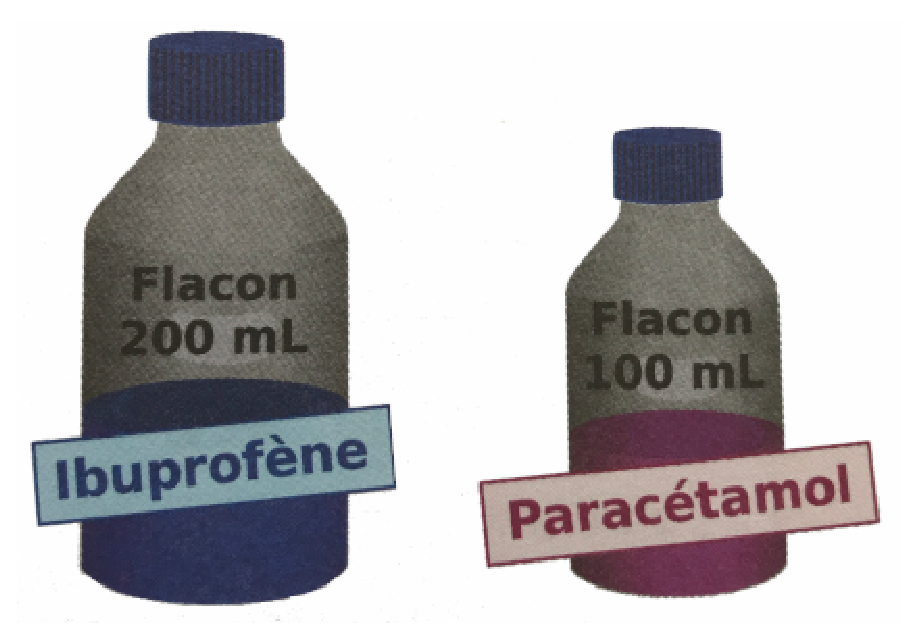
\includegraphics[width=5cm]{medicaments}
%   \end{center}
%   \vspace*{-10mm}
   \begin{enumerate}
      \item Combien de millilitres de sirop contient une prise de paracétamol pour Yanis ?
      \item Combien de millilitres de sirop contient une prise d'ibuprofène pour Yanis ?
      \item Quelle quantité de paracétamol est nécessaire pour soigner Yanis pendant 4 jours ?
      \item Quelle quantité d'ibuprofène est nécessaire pour soigner Yanis pendant 4 jours ?
      \item Combien de jours peut-on traiter Yanis au paracétamol avec un flacon plein de \uml{100} ?
   \end{enumerate}
\end{exercice}

\medskip

\begin{exercice}
   Une marchande fait confectionner 8 douzaines de chemises avec du tissu à \ueuro{3,60} le mètre. L'ouvrière met 8 jours et est payée à raison de \ueuro{68} par jour. Il faut 3 mètres de tissu par chemise. Les fournitures diverses reviennent à \ueuro{99,20} en tout.
   \begin{enumerate}
      \item Quel est le prix de revient pour l'ensemble de la commande ?
       \item Quel est le prix de revient d'une chemise ?
    \end{enumerate}
\end{exercice}

\medskip

\begin{exercice} %10
   Deux échelles la température sont principalement utilisées : l'échelle Celsius et l'échelle Fahrenheit. \\
   La valeur en \degres F d'une température s'obtient en multipliant par 1,8 la température en \degre C et en ajoutant 32.
   \begin{enumerate}
      \item La température de la glace fondante correspond à 0\degres C, combien cela fait-il en \degres F ?
      \item La température d'ébullition de l'eau correspond à 100\degres C, combien cela fait-il en \degres F ?
      \item La météo prévoit une température de 25\degres C pour demain, combien cela fait-il en \degres F ?
      \item Il fait actuellement 40\degres F, à quelle température cela correspond-il en \degres C ?
   \end{enumerate}
\end{exercice}

\end{colonne*exercice}


%%%%%%%%%%%%%%%%%%%%%
%%%%%%%%%%%%%%%%%%%%%
\Recreation

\enigme[Poids et la masse]
   \partie[outre-Terre]
      \begin{minipage}{11.5cm}
         Pourquoi les astronautes peuvent-ils porter plus facilement des objets sur la Lune que sur la Terre ? \\ [2mm]
         \pf \\ [2mm]
         Dans le langage courant on dit : \og Mon poids est de 50 kg \fg{} ou \og Je pèse 50 kg \fg{}. Ces phrases vous paraissent-elle correctes ? \\ [2mm]
         \pf \\ [2mm]
      \end{minipage}
      \qquad
      \begin{minipage}{4.5cm}
         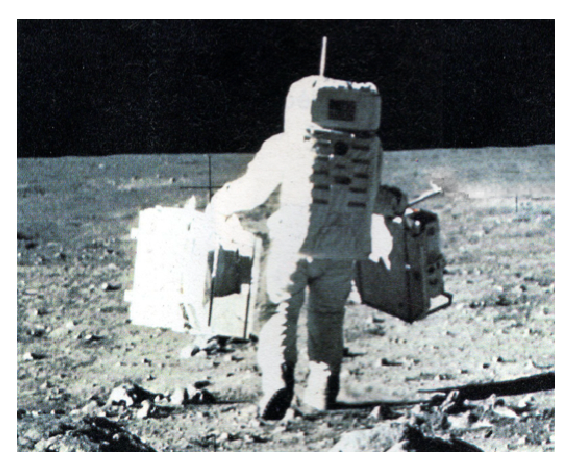
\includegraphics[width=4.5cm]{astronaute}
      \end{minipage}
   
   \partie[poids d'un corps]
      \fbox{Le poids d'un corps est la {\bf force d’attraction} exercée par un corps matériel (Terre, Lune\dots) sur ce corps.} \\ [1mm]
      Cette force d’attraction dépend de la masse du corps et de la masse du corps céleste. La Lune ayant une masse plus petite que celle de la Terre, elle exerce une force plus faible sur un même objet. \\ [2mm]
      Sur la Lune, notre masse change-t-elle ? \pf \\ [2mm]
      Notre poids change-t-il ? \pf \\
   
   \partie[relation entre le poids d'un corps et sa masse]
      On a relevé le poids (exprimé en Newton, de symbole N) et la masse (exprimée en kg) de certains objets sur la Terre et sur la Lune que l'on a représenté dans le graphique cartésien suivant :
      \begin{center}
         {\psset{yunit=0.9}
         \small
         \begin{pspicture}(-1.8,-0.7)(14,6.5)
            \psgrid[gridlabels=0,gridcolor=lightgray](0,0)(12,6)
            \psaxes[dx=1,Dx=10,dy=1,Dy=200]{->}(0,0)(12,6)
            \psline[linecolor=B1](0,0)(12,5.88)
            \rput{26}(6,3.3){\textcolor{B1}{sur la Terre}}
            \psline[linecolor=A1](0,0)(12,0.972)
            \rput{7}(6,0.8){\textcolor{A1}{sur la Lune}}
            \rput[l](12.2,0){\footnotesize\it masse en kg}
            \rput[c](-0.8,5.9){\footnotesize\it poids en N}
         \end{pspicture}}
      \end{center}
      Compléter le tableau suivant :
      \begin{center}
         \begin{tabular}{|p{3.5cm}|*{4}{C{2.4}|}}
            \hline
            Objet & homme & bébé & machine à laver & rugbyman ;-) \\
            \hline
            Masse en kg & 80 & & & \\
            \hline
            Poids en N sur la Terre & & 80 & & 1\,180 \\
            \hline
            Poids en N sur la Lune & & & 120 & \\
            \hline
         \end{tabular}
      \end{center}
      Par combien faut-il multiplier la masse d'un objet en kg pour obtenir son poids en N sur la Terre ? Sur la Lune ? \\ [2mm]
       \pf \\ [2mm]
      Cette constante est appelée accélération de la pesanteur et peut être exprimée en N/kg (Newton par kilogramme).
 
